% 图 78.3 —— 由 `checks/emit_hand.py` 自动拼出（probe 精测 + prims2 图元分解）
%%
% ⚠ 这是**稿子不是成品**：跑 `checks/checkhand.py 78.3` 看指标 + 看叠合图。
%%
%% ⚠ 待核：
%   · 本图 probe 报出阴影族 1 个 —— **本脚本不生成阴影**（要照原书手写）；prims2 的 strokes 里可能含阴影线，核对时留意别画重
%   · 可疑字形 2 项（空心圈 ⊙ 常被认成字母 o）—— 见文件末
%%
\documentclass[12pt]{standalone}
\usepackage{fontspec}
\setsansfont{Arial}
\newfontfamily\mfallback{DejaVu Sans}
\usepackage{tikz}
\usetikzlibrary{arrows.meta}
\begin{document}
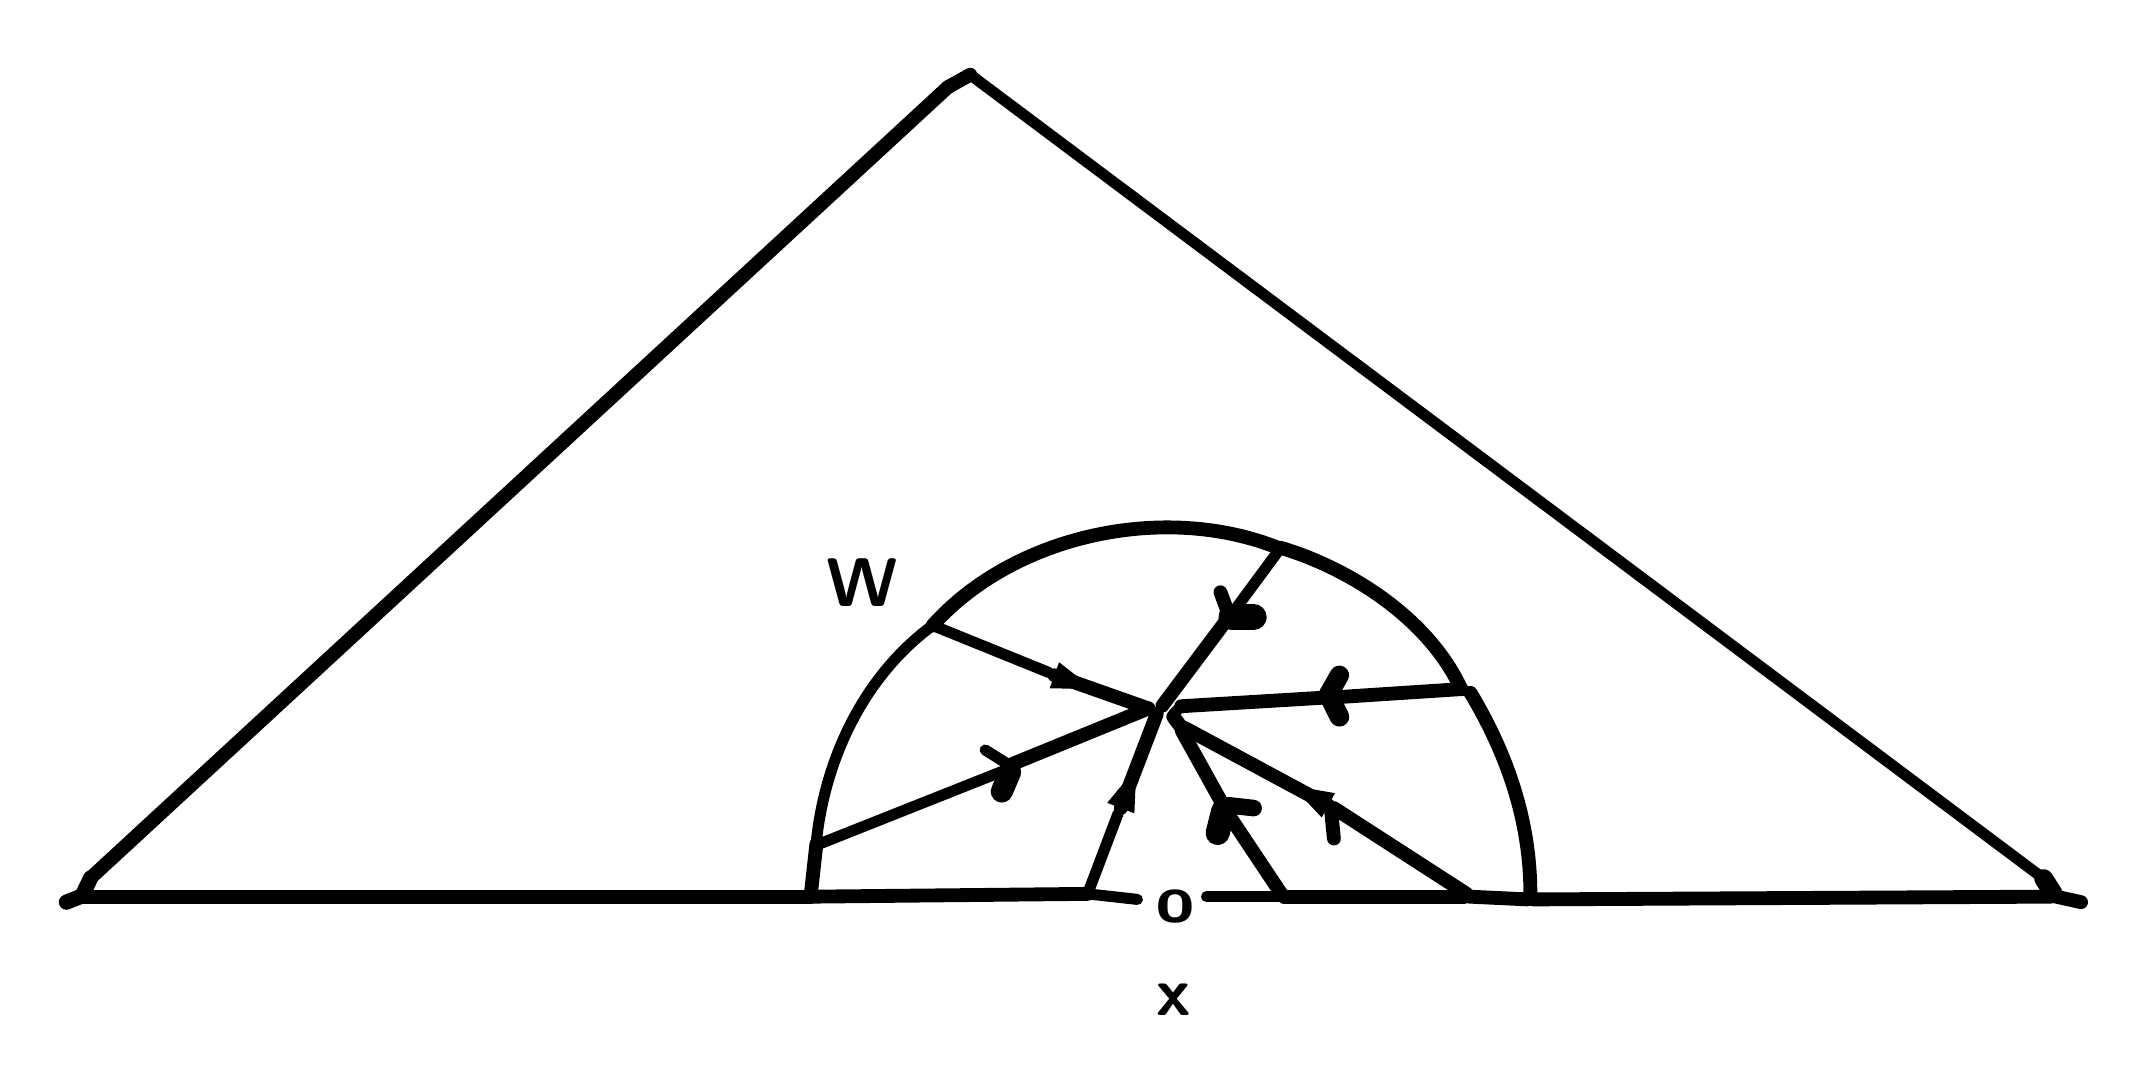
\begin{tikzpicture}[x=1pt, y=-1pt, line width=6.0pt, line cap=round, line join=round]

  %% ════ 直线段（prims2 的 strokes）════
  % （略）线段 (473.0,281.0)-(480.0,277.0) 线宽6.0 —— 是箭头头那一坨，已由箭头头代替
  \draw[line width=3.9pt] (521.4,240.4) -- (518.0,239.0);
  \draw[line width=5.0pt] (434.0,212.0) -- (431.0,204.0);
  \draw[line width=5.0pt] (520.0,313.0) -- (472.0,282.0);
  \draw[line width=8.0pt] (355.0,269.0) -- (352.0,276.0);
  \draw[line width=5.0pt] (544.0,315.0) -- (731.0,314.0);
  \draw[line width=5.0pt] (408.0,248.0) -- (395.0,282.0);
  \fill (399.9,283.9) -- (390.1,280.1) -- (400.6,267.4) -- cycle;
  \draw[line width=5.0pt] (285.0,295.0) -- (283.0,313.0);
  \draw[line width=4.0pt] (426.0,314.0) -- (452.0,314.0);
  \draw[line width=9.4pt] (435.0,213.0) -- (443.0,213.0);
  \draw[line width=5.0pt] (432.0,281.0) -- (417.0,254.0);
  \draw[line width=6.8pt] (732.0,313.0) -- (728.5,307.5);
  \draw[line width=4.0pt] (728.5,307.5) -- (340.6,17.0);
  \draw[line width=5.0pt] (340.6,17.0) -- (332.5,21.5);
  \draw[line width=5.0pt] (332.5,21.5) -- (22.8,307.2);
  \draw[line width=5.5pt] (22.8,307.2) -- (20.0,313.0);
  % （略）线段 (386.0,285.0)-(393.0,283.0) 线宽7.7 —— 是箭头头那一坨，已由箭头头代替
  \draw[line width=4.0pt] (452.0,189.0) -- (435.0,212.0);
  \draw[line width=5.0pt] (471.0,283.0) -- (472.0,293.0);
  \draw[line width=5.0pt] (418.0,253.0) -- (470.0,281.0);
  \fill (472.4,276.6) -- (467.6,285.4) -- (456.8,273.9) -- cycle;
  \draw[line width=6.0pt] (434.0,281.0) -- (443.0,282.0);
  \draw[line width=5.5pt] (19.0,314.0) -- (14.0,316.0);
  \draw[line width=4.0pt] (369.0,233.0) -- (327.0,216.0);
  \draw[line width=4.0pt] (354.0,268.0) -- (286.0,295.0);
  \draw[line width=5.0pt] (742.0,316.0) -- (733.0,314.0);
  \draw[line width=5.0pt] (284.0,314.0) -- (383.0,313.0);
  % （略）线段 (370.0,232.0)-(367.0,223.0) 线宽9.9 —— 是箭头头那一坨，已由箭头头代替
  \draw[line width=5.0pt] (453.0,313.0) -- (433.0,283.0);
  \draw[line width=4.0pt] (414.0,248.0) -- (416.8,245.2);
  \draw[line width=5.0pt] (416.8,245.2) -- (470.0,242.0);
  \draw[line width=8.7pt] (432.0,283.0) -- (430.0,291.0);
  % （略）线段 (363.0,238.0)-(369.0,234.0) 线宽7.6 —— 是箭头头那一坨，已由箭头头代替
  \draw[line width=4.0pt] (394.0,284.0) -- (383.0,313.0);
  \draw[line width=4.0pt] (346.0,261.0) -- (354.0,266.0);
  \draw[line width=5.0pt] (434.0,213.0) -- (410.0,245.0);
  \draw[line width=5.0pt] (519.0,314.0) -- (454.0,314.0);
  \draw[line width=5.0pt] (472.0,242.0) -- (518.0,239.0);
  \draw[line width=5.1pt] (417.0,253.0) -- (414.0,249.0);
  \draw[line width=5.0pt] (356.0,266.0) -- (405.0,246.0);
  \draw[line width=5.0pt] (405.0,246.0) -- (371.0,234.0);
  \fill (369.3,238.7) -- (372.7,229.3) -- (385.1,239.0) -- cycle;
  \draw[line width=5.0pt] (521.0,314.0) -- (542.0,315.0);
  \draw[line width=4.0pt] (383.0,313.0) -- (401.0,315.0);
  % （略）线段 (399.0,290.0)-(395.0,284.0) 线宽7.6 —— 是箭头头那一坨，已由箭头头代替
  \draw[line width=7.0pt] (474.0,234.0) -- (470.0,241.0);
  \draw[line width=7.1pt] (474.0,249.0) -- (471.0,243.0);
  \draw[line width=5.0pt] (283.0,314.0) -- (20.0,314.0);

  %% ════ 曲线（prims2 的 curves —— 三段式，坐标同为 (y,x)）════
  \draw[line width=5.0pt] (543.0,314.0) .. controls (543.2,287.2) and (534.8,262.8) .. (521.4,240.4);
  \draw[line width=5.0pt] (452.0,188.0) .. controls (410.8,171.5) and (356.4,183.2) .. (327.0,216.0);
  \draw[line width=5.0pt] (453.0,188.0) .. controls (478.5,195.7) and (506.5,213.9) .. (518.0,239.0);
  \draw[line width=4.0pt] (327.0,216.0) .. controls (302.1,234.3) and (288.1,264.3) .. (285.0,294.0);

  %% ════ 标签（probe 直接给的 \node 行）════
  %% ⚠ 全部补了 fill=white：文字在最上层，否则与曲线交叉干扰
     \node[anchor=center,inner sep=0pt,fill=white,font=\fontsize{28.0}{35.0}\selectfont] at (301.7,200.4) {\textsf{\textbf{\textit{W}}}};   % box(289,189,25,21)
     \node[anchor=center,inner sep=0pt,fill=white,font=\fontsize{33.2}{41.5}\selectfont] at (414.8,317.7) {\textsf{\textbf{\textit{o}}}};   % box(405,307,18,18)
     \node[anchor=center,inner sep=0pt,fill=white,font=\fontsize{29.2}{36.5}\selectfont] at (414.0,351.4) {\textsf{\textbf{\textit{x}}}};   % box(405,341,16,17)

  % 钉死画布：否则超出的图元/控制点会把页面撑大，1:1 回比就失准
  \pgfresetboundingbox
  \path[use as bounding box] (0,0) rectangle (751,365);
\end{tikzpicture}
\end{document}

% ⚠ 待核清单（probe 拿不准，人眼过一遍）：
%   · 可疑字形：\node[anchor=center,inner sep=0pt,font=\fontsize{33.2}{41.5}\selectfont] at (414.8,317.7) {\textsf{\textbf{\te
%   · 未识别/跳过：⑤ 跳过/未识别的字形
